\documentclass[12pt]{article}

\usepackage{amsmath}
\usepackage{amssymb}
\usepackage{calc}
\usepackage{units}
\usepackage{graphicx}
\usepackage[pdftex]{hyperref}
\usepackage{subfig}
\usepackage[margin=1in]{geometry}
\usepackage{listings}
\usepackage[numbers,sort&compress]{natbib}
\usepackage{bm}
\usepackage{paralist}
\usepackage[draft]{fixme}
\usepackage{textcomp}
\usepackage{yorkdefs}

\newcommand{\Sone}{\ensuremath{S_1}\xspace}
\newcommand{\Stwo}{\ensuremath{S_2}\xspace}

\hypersetup{
  breaklinks=true,
  pdftitle={Refraction and Dispersion},
  pdfauthor={Kevin R. Lynch},
  pdfsubject={Phyiscs, Electricity and magnetism, Optics},
  pdfkeywords={refraction, dispersion},
  pdflang={en-US},
}

\title{Refraction and Dispersion}
\author{}
%Kevin R. Lynch
%\date{2012-04-20}
\date{}

\begin{document}

\maketitle

\section{Objectives}
\label{sec:objectives}

\begin{enumerate}
\item To understand refraction in optical systems, and
\item To understand dispersion in optical systems.
\end{enumerate}

\section{Introduction}
\label{sec:introduction}

From Einstein's Special Theory of Relativity, we learn that the
maximum speed at which any object or information can travel is that of
the speed of light in vacuum, usually denoted as $c$.  Light traveling
in any other medium travels at less than this speed.  Because light
must change speed when it crosses the boundary between materials, rays
of light \textit{refract}, or change direction.  Further, the
refractory properties of materials are different at different
wavelengths; this frequency dependent behavior is known as
\textit{dispersion}.  We will study both behaviors in this lab.

\section{Theory}
\label{sec:theory}

You learned in PHYS-151 that when a phenomenon is governed by the wave
equation 
\begin{gather*}
  \pderiv[2]{A(x,t)}{t} = v^2 \pderiv[2]{A(x,t)}{x}\ ,
\end{gather*}
the resulting wave trains are governed by a simple law
\begin{gather*}
  v = \lambda f\ ,
\end{gather*}
that is, the speed of wave propagation equals the product of the
frequency and the wavelength.  Einstein argued, and the data has
repeatedly borne out the prediction, that the speed of light in a
vacuum, $c = \unit[299\, 792\, 458]{\nicefrac{m}{s}}$ exactly, is a
universal constant for all observers.  It is also a universal speed
\textit{limit}: nothing can travel faster than light in a vacuum.  But
that doesn't mean that light \textit{always} travels at the speed $c$;
in fact, in different materials, the propagation speed of light, $v$,
is less (sometimes significantly!) than this.  We define the
\textit{index of refraction} of a material as the ratio of $c$ to $v$:
\begin{gather*}
  n = \frac{c}{v}\ ,
\end{gather*}
and these values are always positive\footnote{You can, in fact,
  engineer \textit{metamaterials} with negative indices in certain
  frequency bands; no such materials have ever been found in nature.}
and greater than 1.  The refractive index of vacuum is exactly 1,
while the refractive index of dry air at STP is so close to 1
($1.000\, 293$) as to be indistinguishable in our labs.  Your text
lists the indices for a number of other materials, some with $n>2$.

\begin{figure}
  \centering
  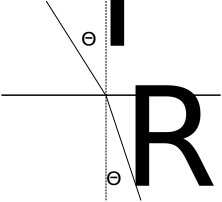
\includegraphics[width=\textwidth/3]{figures/refraction}  
  \caption{The definition of the incident and refracted angles.  Light
    enters the interface at an angle $\theta_I$ with respect to the
    normal to the surface, and leaves the interface at an angle
    $\theta_R$.  If $\theta_I \neq \theta_R$, then the ray is said to
    be refracted.}
  \label{fig:defs}
\end{figure}
The frequency of the wave train is simply the number of cycles per
unit time, and continuity requires that this value doesn't change at
an interface between materials of different indices.  As a consequence
the \textit{wavelength} of the wave must change across the boundary,
and that can only happen if the wave changes direction!  Because the
different components of the reflected and refracted waves must add up
to the total incoming wave, you can find a relationship between the
angles of the incident and refracted rays (defined in
Figure~\ref{fig:defs})
\begin{gather*}
  \frac{\sin \theta_I}{\sin \theta_R} = \frac{v_I}{v_R}.
\end{gather*}
Rewriting the $v_i$ in terms of the $n_i$ gives
\begin{gather*}
  n_I \sin\theta_I = n_R \sin\theta_R\ ,
\end{gather*}
famously known as \textit{Snell's Law} of refraction.  If light slows
down when crossing a boundary (a transition from low to high $n$), the
rays bend towards the normal, and vice versa.  You will use Snell's
Law to determine the speed of light in different materials.

% Total Internal Reflection
\begin{figure}
  \centering
  \subfloat[][Dispersion Curves]{
%% Figure under Gnu Free Documentation License
%% http://en.wikipedia.org/wiki/File:Dispersion-curve.png
    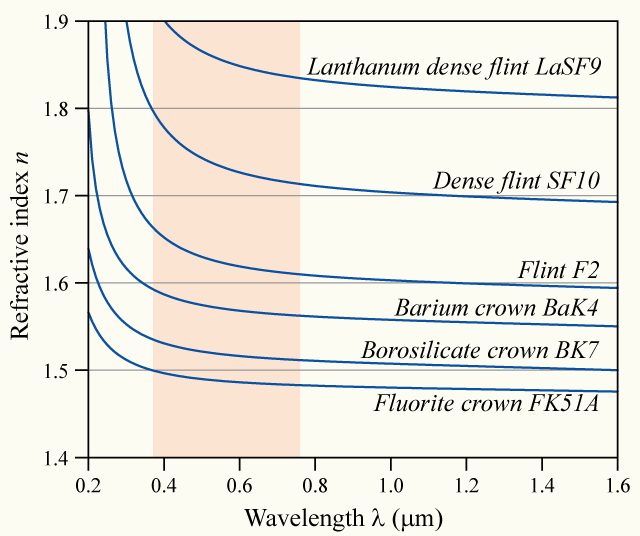
\includegraphics[width=\textwidth/2-0.1in]{figures/Dispersion-curve}
  }
  \subfloat[][Rainbows]{
%% File in public domain
%% http://en.wikipedia.org/wiki/File:Rainbow1.svg
    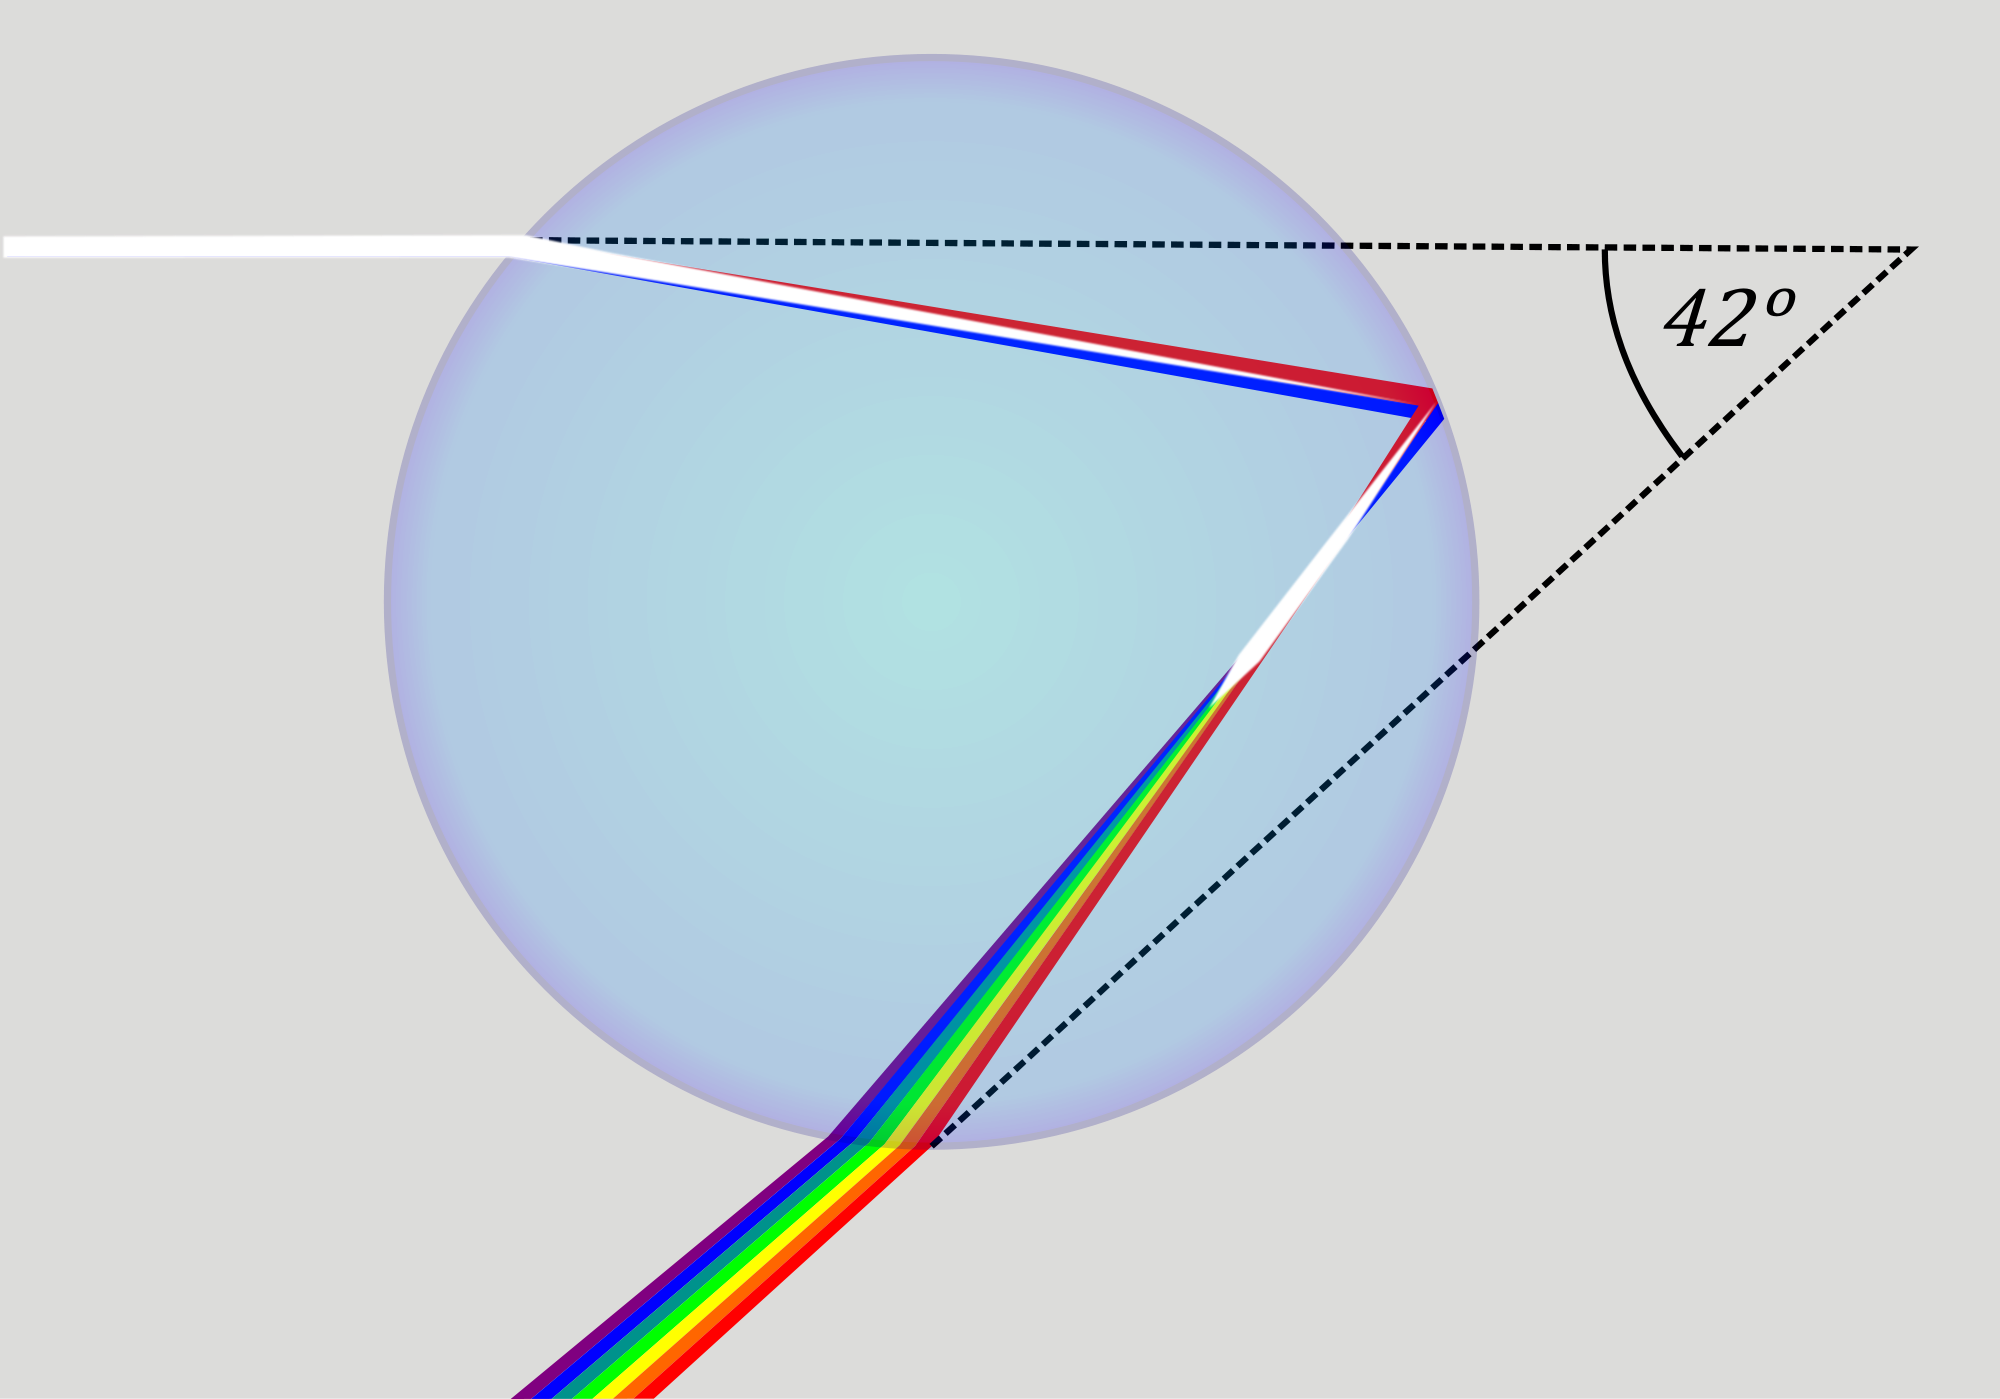
\includegraphics[width=\textwidth/2-0.1in]{figures/Rainbow1}
  }
  \caption{The left-hand image shows the dispersion curves (wavelength
  vs index) for a number of different types of optical glass.  The
  right-hand image show the process in a raindrop that creates a
  rainbow: a pair of dispersive refractions, with an intervening
  internal reflection.}
  \label{fig:dispersion}
\end{figure}

While the discussion above has repeatedly talked about \textit{the}
index of refraction of a material, it turns out there really is no
such thing: the index of refraction depends on the frequency of the
light!  That is, we really have to replace relation $v = \lambda f$
with
\begin{gather*}
  v(f) = \lambda f\ .
\end{gather*}
This more complicated relationship is known as a \textit{dispersion
  relation}, and gives rise to frequency dependent refraction known as
dispersion.  While the difference from a constant speed is usually
very small (often less than a percent across the optical frequencies,
see Figure~\ref{fig:dispersion}), it has a host of very well known
consequences, the most interesting of which are the \textit{chromatic
  aberration} of camera systems, and the formation of rainbows (again,
see Figure~\ref{fig:dispersion}).  You will also explore dispersion in
this lab.

\section{Procedures}
\label{sec:procedures}

You will receive a number of clear blocks, laser pointers,
protractors, white paper, and tape measures and meter sticks.  You
must use the information below to design and implement a series of
experiments to measure refraction and dispersion in optical systems. 

\subsection{Index of Refraction}
\label{sec:index}

In the first two measurements, you'll be using Snell's Law to
determine the index of refraction of two acrylic objects.  Typically,
these measurements in an undergraduate lab are taken with collimated
white light sources, where dispersion and divergence conspire to
complicate the measurements.  Instead, we will use monochromatic,
non-divergent light sources: diode based laser pointers; the rays
consist of a single wavelength with a very small beam spread.  You
should be able to make excellent measurements with a modicum of care.

\subsubsection{Acrylic Cube}
\label{sec:cube}

\begin{figure}
  \centering
  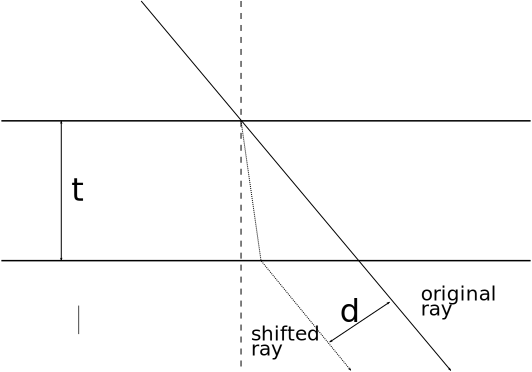
\includegraphics[width=\textwidth/2]{figures/slab}
  \caption{The offset distance, $d$, between the original ray and the
    refracted ray after passing through a slab of thickness $t$.}
  \label{fig:cube}
\end{figure}

A ray from a laser will travel across the lab in a straight line.  If
you intersect the beam with a slab with index of refraction $n$ and
parallel sides, the ray that emerges will be parallel to the original
ray, but offset by a distance $d$; see Figure~\ref{fig:cube}.  By
measuring incident angle $\theta_I$ and the offset distance $d$, you
can extract the index of refraction.

Determine how to make this measurement.  You must make a very careful
measurement - the uncertainty of your result is very sensitive to the
uncertainty of your angular measurements.  While you have protractors
available to you, and you should use them to sanity check your
measurements, by themselves they won't give you good enough results.

\subsubsection{Acrylic Prism}
\label{sec:prism}

\begin{figure}
  \centering
  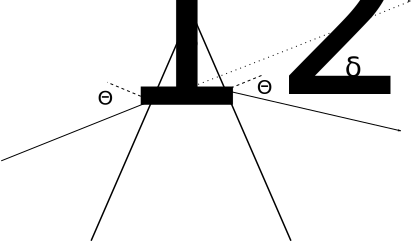
\includegraphics[width=\textwidth/2]{figures/prism}
  \caption{The angle of deviation, $\delta$, for a ray passing through
    a prism.  Light enters the interface at an angle $\theta_1$ with
    respect to the normal to the surface, and leaves the interface at
    an angle $\theta_2$.  If $\theta_1 = \theta_2$, then $\delta$ is a
    minimum.}
  \label{fig:prism}
\end{figure}

The \textit{prism} is a triangular block of dispersive material,
typically used to break a light source with multiple wavelengths into
its constituent parts, much like a diffraction grating.  They are also
used in optical systems (such as cameras and periscopes) to transport
or split images.  Here, you'll use the prism to determine the index of
refraction of the prism material.

Figure~\ref{fig:prism} shows how the path of light is deflected when
passing through the prism.  This deflection angle is called the
\textit{angle of deviation}.  The minimum angle $\delta_\mathrm{min}$
occurs when the incoming and outgoing deflection angles are
equal.\footnote{You could consider proving this\ldots} At this angle,
the index of the prism material is given by
\begin{gather*}
  n = \frac{\sin\left(\frac{\Phi+\delta_\mathrm{min}}{2}\right)}
  {\sin\left(\frac{\Phi}{2}\right)}\ ,
\end{gather*}
assuming the prism is in air.

Measure the index of refraction for the prism.  You can certainly use
the minimum angle of deviation method.  Additionally, there is a one
angle measurement that gives the same information.  What is that
method?

% \fixme{Total Internal Reflection}

\subsection{Dispersion}
\label{sec:dispersion}

Acrylic polymers are well matched to optical transmission, because
their dispersion curves are relatively constant across optical
wavelengths.  Still, with sufficient care, observation of dispersion
is not difficult.  Here, you will receive three different colored
laser pointers and a number of acrylic blocks; devise an experiment to
prove that these different frequencies travel at different speeds
through the acrylic.

\newpage
 
\section*{Pre-Lab Exercises}

Answer these questions as instructed on Blackboard; make sure to
submit them before your lab session!

\begin{enumerate}
\item A ray hits an object at 15\textdegree\  from the vertical.  If the
  material has index of refraction 1.5, what is the refraction angle?
% 9.9\textdegree
\item If a ray is incident on a block of material at 15\textdegree\ 
  from the vertical, and is refracted to 8\textdegree\  from the
  vertical, what is the index of refraction?
% 1.86
\item  A ray of light crosses from a flint glass slab at
  20\textdegree\  from the normal into air.  At what angle does it
  emerge? 
% 35\textdegree
\item A ray of light passes through a prism, making the minimum angle
  of deviation.  The rays enter and emerge at 7\textdegree\ from the
  normal to the surface.  What is the index of refraction of the
  material, if the prism angle is 50\textdegree?
% 1.1
\end{enumerate}

\newpage

\section*{Post-Lab Exercises}

\begin{enumerate}
\item What measurement did you devise in Section~\ref{sec:cube}?  What
  is the index of refraction for you laser in the acrylic?  What does
  this give as the speed of light in the acrylic?  Estimate the
  uncertainty of your result.
\item What measurement did you devise in Section~\ref{sec:prism}?
  What is the index of refraction for you laser in the acrylic?  What
  does this give as the speed of light in the acrylic?  Estimate the
  uncertainty of your result.
\item What experiment did you devise in Section~\ref{sec:dispersion}?
  How does your data prove that different wavelengths travel at
  different speeds through the material?  What are the corresponding
  speeds of light in the acrylic?  Estimate the uncertainty of your
  result.
\item Discuss briefly whether you have met the objectives of the lab
  exercises.
\end{enumerate}

\end{document}

%%% Local Variables: 
%%% mode: latex
%%% TeX-master: t
%%% End: 
